\begin{enumerate}[label=\thesubsection.\arabic*, ref=\thesubsection.\theenumi,itemsep=0pt]

\item If $\vec{a}, \vec{b}, \vec{c}$ are the position vectors of the points $A\brak{2,3,-4}$, $B\brak{3,-4,-5}$ and $C\brak{3,2,-3}$ respectively, then $\norm{\vec{a}+\vec{b}+\vec{c}}$ is equal to
\hfill (CBSE XII 65/C/3, Q1)
\begin{enumerate}[itemsep=0pt]
\begin{multicols}{4}
\item $\sqrt{113}$
\item $\sqrt{185}$
\item $\sqrt{203}$
\item $\sqrt{209}$
\end{multicols}
\end{enumerate}

\solution
\begin{align}
\vec{a}+\vec{b}+\vec{c} = \myvec{2 \\ 3 \\ -4} + \myvec{3 \\ -4 \\ -5} + \myvec{3 \\ 2 \\ -3} = \myvec{8 \\ 1 \\ -12}
\end{align}
From \eqref{eq:cb12-dot}, $\norm{\vec{a}+\vec{b}+\vec{c}}^2 = 64 + 1 + 144 = 209$. Hence option (D). The following code verifies this.
\begin{lstlisting}[frame=single, basicstyle=\rmfamily, escapeinside={(*@}{@*)}]
(*@\makebox[\dimexpr\linewidth-2\fboxsep-2\fboxrule\relax][c]{codes/q1.py}@*)
\end{lstlisting}

\item The distance between the planes $4x - 4y + 2z + 5 = 0$ and $2x - 2y + z + 6 = 0$ is
\hfill (CBSE XII 65/C/3, Q3)
\begin{enumerate}[itemsep=0pt]
\begin{multicols}{4}
\item $\frac{1}{6}$
\item $\frac{7}{6}$
\item $\frac{11}{6}$
\item $\frac{16}{6}$
\end{multicols}
\end{enumerate}

\solution In the form $\vec{n}^{\top}\vec{x} = c$: $\vec{n}_1 = \myvec{4 \\ -4 \\ 2}$, $c_1 = -5$ and $\vec{n}_2 = \myvec{2 \\ -2 \\ 1}$, $c_2 = -6$. Since $\vec{n}_1 = 2\vec{n}_2$ the planes are parallel. From \eqref{eq:cb12-planes} with $\lambda = 2$,
\begin{align}
d = \frac{\abs{-5 - 2\brak{-6}}}{\norm{\vec{n}_1}} = \frac{7}{\sqrt{16+16+4}} = \frac{7}{6}
\end{align}
Hence option (B). The following code verifies this.
\begin{lstlisting}[frame=single, basicstyle=\rmfamily, escapeinside={(*@}{@*)}]
(*@\makebox[\dimexpr\linewidth-2\fboxsep-2\fboxrule\relax][c]{codes/q3.py}@*)
\end{lstlisting}

\item The probabilities of solving a specific question independently by $A$ and $B$ are $\frac{1}{3}$ and $\frac{1}{5}$ respectively. If both try to solve the question independently, the probability that the question is solved is
\hfill (CBSE XII 65/C/3, Q4)
\begin{enumerate}[itemsep=0pt]
\begin{multicols}{4}
\item $\frac{7}{15}$
\item $\frac{8}{15}$
\item $\frac{2}{15}$
\item $\frac{14}{15}$
\end{multicols}
\end{enumerate}

\solution The pmfs of $A$ and $B$ (index $0$: fails, $1$: solves) are $p_A = \myvec{\frac{2}{3} \\ \frac{1}{3}}$, $p_B = \myvec{\frac{4}{5} \\ \frac{1}{5}}$. By independence, from \eqref{eq:cb12-pmf} the joint pmf is
\begin{align}
p_{AB} = p_Ap_B^{\top} = \myvec{\frac{8}{15} & \frac{2}{15} \\ \frac{4}{15} & \frac{1}{15}}
\end{align}
The question is solved unless both fail, so $\pr{\text{solved}} = 1 - \frac{8}{15} = \frac{7}{15}$. Hence option (A). The following code verifies this.
\begin{lstlisting}[frame=single, basicstyle=\rmfamily, escapeinside={(*@}{@*)}]
(*@\makebox[\dimexpr\linewidth-2\fboxsep-2\fboxrule\relax][c]{codes/q4.py}@*)
\end{lstlisting}

\item If $\sec^{-1}\brak{\dfrac{1+x}{1-y}} = a$, then $\dfrac{dy}{dx}$ is equal to
\hfill (CBSE XII 65/C/3, Q6)
\begin{enumerate}[itemsep=0pt]
\begin{multicols}{4}
\item $\frac{x-1}{y-1}$
\item $\frac{x-1}{y+1}$
\item $\frac{y-1}{x+1}$
\item $\frac{y+1}{x-1}$
\end{multicols}
\end{enumerate}

\solution Let $k = \sec a$ (a constant). Then $\frac{1+x}{1-y} = k$, i.e.
\begin{align}
y = 1 - \frac{1+x}{k}
\end{align}
Take $x \to t$. By \eqref{eq:cb12-laplace},
\begin{align}
Y(s) = \frac{1}{s} - \frac{1}{k}\brak{\frac{1}{s^2} + \frac{1}{s}}, \quad y(0) = 1 - \frac{1}{k}
\end{align}
From \eqref{eq:cb12-lap1},
\begin{align}
L\{y'\}(s) &= sY(s) - y(0) = 1 - \frac{1}{ks} - \frac{1}{k} - 1 + \frac{1}{k} = -\frac{1}{k}\cdot\frac{1}{s} = L\cbrak{-\frac{1}{k}} \\
\implies \frac{dy}{dx} &= -\frac{1}{k} = -\frac{1-y}{1+x} = \frac{y-1}{x+1}
\end{align}
Hence option (C). The following code checks the Laplace relation numerically with $a = 1$ rad (assumed), the Euler forward difference \eqref{eq:cb12-euler-diff} and the four options.
\begin{lstlisting}[frame=single, basicstyle=\rmfamily, escapeinside={(*@}{@*)}]
(*@\makebox[\dimexpr\linewidth-2\fboxsep-2\fboxrule\relax][c]{codes/q6.py}@*)
\end{lstlisting}

\item $\displaystyle\int_0^1 \tan\brak{\sin^{-1}x}\,dx$ equals
\hfill (CBSE XII 65/C/3, Q9)
\begin{enumerate}[itemsep=0pt]
\begin{multicols}{4}
\item 2
\item 0
\item $-1$
\item 1
\end{multicols}
\end{enumerate}

\solution Put $x = \sin\theta$, $dx = \cos\theta\,d\theta$, $\theta \in \sbrak{0, \frac{\pi}{2}}$. Then $\tan\theta\cos\theta = \sin\theta$ and
\begin{align}
\int_0^1 \tan\brak{\sin^{-1}x}\,dx = \int_0^{\pi/2}\sin\theta\,d\theta
\end{align}
The trapezoidal rule \eqref{eq:cb12-trap} gives $0.99794$ for $N = 10$, $0.99998$ for $N = 100$ and $1.00000$ for $N = 10^4$, so the value is $1$ (exactly $\sbrak{-\cos\theta}_0^{\pi/2} = 1$). Hence option (D). The following code verifies this.
\begin{lstlisting}[frame=single, basicstyle=\rmfamily, escapeinside={(*@}{@*)}]
(*@\makebox[\dimexpr\linewidth-2\fboxsep-2\fboxrule\relax][c]{codes/q9.py}@*)
\end{lstlisting}

\item The roots of the equation $\mydet{x & 0 & 8 \\ 4 & 1 & 3 \\ 2 & 0 & x} = 0$ are
\hfill (CBSE XII 65/C/3, Q10)
\begin{enumerate}[itemsep=0pt]
\begin{multicols}{4}
\item $-4, 4$
\item $2, -4$
\item $2, 4$
\item $2, 8$
\end{multicols}
\end{enumerate}

\solution Expanding along the second column, which has a single non-zero entry,
\begin{align}
\mydet{x & 0 & 8 \\ 4 & 1 & 3 \\ 2 & 0 & x} = 1\cdot\mydet{x & 8 \\ 2 & x} = x^2 - 16 = 0
\end{align}
The roots are found by the Newton-Raphson iteration \eqref{eq:cb12-nr}
\begin{align}
x_{n+1} = x_n - \frac{x_n^2 - 16}{2x_n} = \frac{1}{2}\brak{x_n + \frac{16}{x_n}}
\end{align}
which converges to $4$ from $x_0 = 5$ and to $-4$ from $x_0 = -5$. Hence option (A). The following code evaluates the determinant by cofactor expansion and finds the roots.
\begin{lstlisting}[frame=single, basicstyle=\rmfamily, escapeinside={(*@}{@*)}]
(*@\makebox[\dimexpr\linewidth-2\fboxsep-2\fboxrule\relax][c]{codes/q10.py}@*)
\end{lstlisting}

\item A square matrix $\vec{A}$ is said to be singular if \underline{\hspace{1.5cm}}.
\hfill (CBSE XII 65/C/3, Q11)

\hfill OR \\
If $\vec{A} = \myvec{3 & -5 \\ 2 & 0}$ and $\vec{B} = \myvec{1 & 17 \\ 0 & -10}$, then $\mydet{\vec{A}\vec{B}} = $ \underline{\hspace{1.5cm}}.

\solution From \eqref{eq:cb12-det}, $\vec{A}$ is singular if $\mydet{\vec{A}} = 0$. 

\textbf{OR:} $\mydet{\vec{A}} = 0 - \brak{-10} = 10$, $\mydet{\vec{B}} = -10$, so
\begin{align}
\mydet{\vec{A}\vec{B}} = \mydet{\vec{A}}\mydet{\vec{B}} = -100
\end{align}
(directly, $\vec{A}\vec{B} = \myvec{3 & 101 \\ 2 & 34}$ and $3\cdot 34 - 101\cdot 2 = -100$). The following code verifies this.
\begin{lstlisting}[frame=single, basicstyle=\rmfamily, escapeinside={(*@}{@*)}]
(*@\makebox[\dimexpr\linewidth-2\fboxsep-2\fboxrule\relax][c]{codes/q11.py}@*)
\end{lstlisting}

\item A card is picked at random from a pack of $52$ playing cards. Given that the picked up card is a queen, the probability of it being a queen of spades is \underline{\hspace{1.5cm}}.
\hfill (CBSE XII 65/C/3, Q13)

\solution Each card has pmf $\frac{1}{52}$. Let $Q$ be the event that the card is a queen and $QS$ the queen of spades. $\pr{Q} = \frac{4}{52}$, $\pr{QS\,Q} = \frac{1}{52}$. From \eqref{eq:cb12-cond},
\begin{align}
\pr{QS|Q} = \frac{1/52}{4/52} = \frac{1}{4}
\end{align}
Given a queen, the four queens are equally likely. The following code verifies this.
\begin{lstlisting}[frame=single, basicstyle=\rmfamily, escapeinside={(*@}{@*)}]
(*@\makebox[\dimexpr\linewidth-2\fboxsep-2\fboxrule\relax][c]{codes/q13.py}@*)
\end{lstlisting}

\item The integrating factor of the differential equation $x\dfrac{dy}{dx} - y = \log x$ is \underline{\hspace{1.5cm}}.
\hfill (CBSE XII 65/C/3, Q14)

\solution In the standard form $\frac{dy}{dx} - \frac{1}{x}y = \frac{\log x}{x}$, so from \ref{eq:cb12-linode},
\begin{align}
\text{IF} = e^{-\int \frac{dx}{x}} = \frac{1}{x}
\end{align}
\textbf{Laplace transform:} put $x = e^t$. Then $x\frac{dy}{dx} = \frac{dy}{dt}$ and the equation becomes $\frac{dy}{dt} - y = t$. From \eqref{eq:cb12-lap1} and \eqref{eq:cb12-laplace},
\begin{align}
sY - y_0 - Y = \frac{1}{s^2} \implies Y(s) = \frac{y_0}{s-1} + \frac{1}{s^2\brak{s-1}}
\end{align}
Here the integrating factor in $t$ is $e^{-t} = \frac{1}{x}$, and the solution is $y = -\brak{\log x + 1} + Cx$ with $C = y_0 + 1$. The IF makes the left side exact, $\frac{d}{dx}\brak{\frac{y}{x}} = \frac{xy' - y}{x^2} = \frac{\log x}{x^2}$, which the code checks with the Euler forward difference \eqref{eq:cb12-euler-diff}. The code also compares the numerical Laplace transform of $y(t)$ with $Y(s)$ and solves the ODE by the Euler forward method \eqref{eq:cb12-euler} in \figref{fig:cb12-q14}.
\begin{lstlisting}[frame=single, basicstyle=\rmfamily, escapeinside={(*@}{@*)}]
(*@\makebox[\dimexpr\linewidth-2\fboxsep-2\fboxrule\relax][c]{codes/q14.py}@*)
\end{lstlisting}
\begin{figure}[H]
\centering
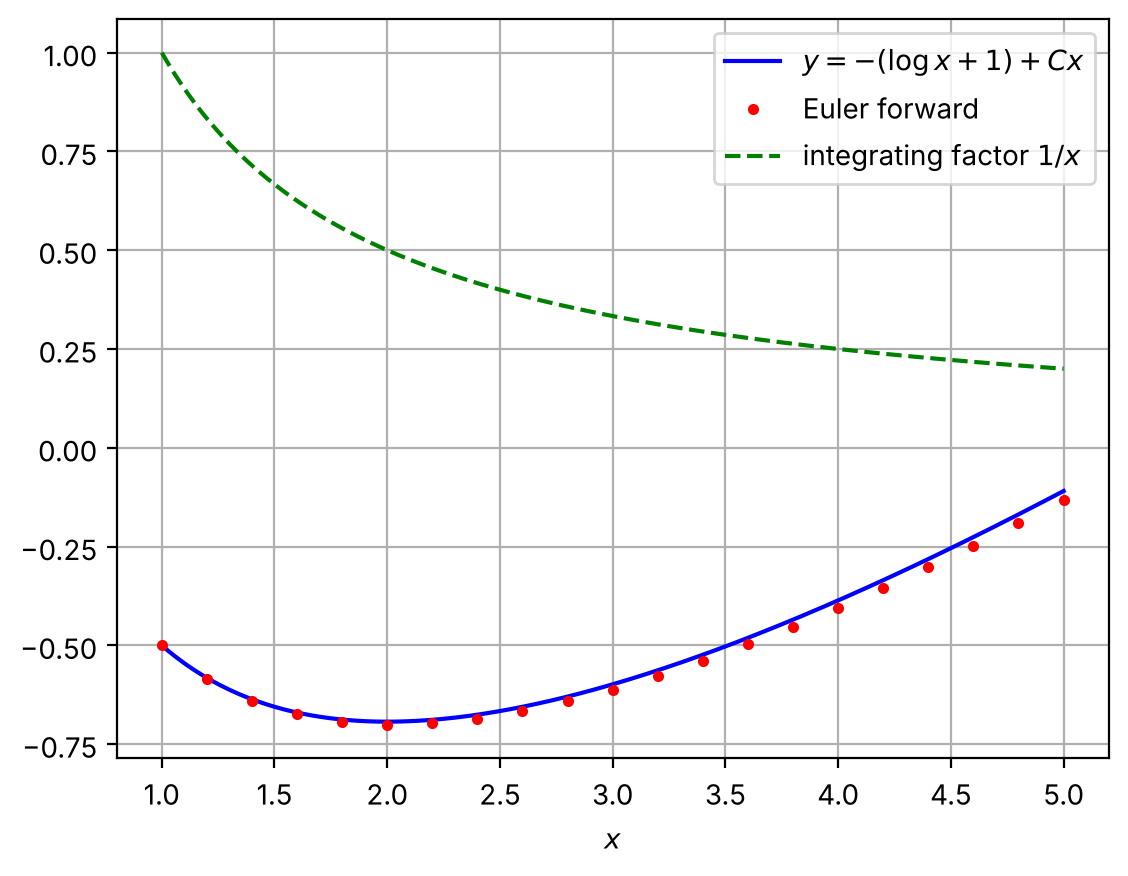
\includegraphics[width=0.65\linewidth]{figs/q14.png}
\caption{Solution, Euler forward method and the integrating factor $1/x$}
\label{fig:cb12-q14}
\end{figure}

\item If $y = \log x$, then $\dfrac{d^2y}{dx^2} = $ \underline{\hspace{1.5cm}}.
\hfill (CBSE XII 65/C/3, Q15)

\solution $y' = \frac{1}{x}$ and $y'' = -\frac{1}{x^2}$. 

\textbf{Laplace transform:} with $t = x - 1$, $y\brak{t} = \log\brak{1+t}$, $y(0) = 0$, $y'(0) = 1$. From \eqref{eq:cb12-lap1} and \eqref{eq:cb12-lap2},
\begin{align}
L\{y'\} = sY(s), \quad L\{y''\} = s^2Y(s) - 1
\end{align}
The code computes $Y(s)$ with the trapezoidal rule and finds, e.g. at $s = 2$, $L\{y'\} = 0.361329$ against $sY = 0.361329$ for $y' = \frac{1}{1+t}$, and $L\{y''\} = -0.277343$ against $s^2Y - 1 = -0.277343$ for $y'' = -\frac{1}{\brak{1+t}^2}$. The Euler second difference \eqref{eq:cb12-euler-diff} gives $-0.9998, -0.2500, -0.0625$ at $x = 1, 2, 4$ which are $-\frac{1}{x^2}$. Hence
\begin{align}
\frac{d^2y}{dx^2} = -\frac{1}{x^2}
\end{align}
See \figref{fig:cb12-q15}.
\begin{lstlisting}[frame=single, basicstyle=\rmfamily, escapeinside={(*@}{@*)}]
(*@\makebox[\dimexpr\linewidth-2\fboxsep-2\fboxrule\relax][c]{codes/q15.py}@*)
\end{lstlisting}
\begin{figure}[H]
\centering
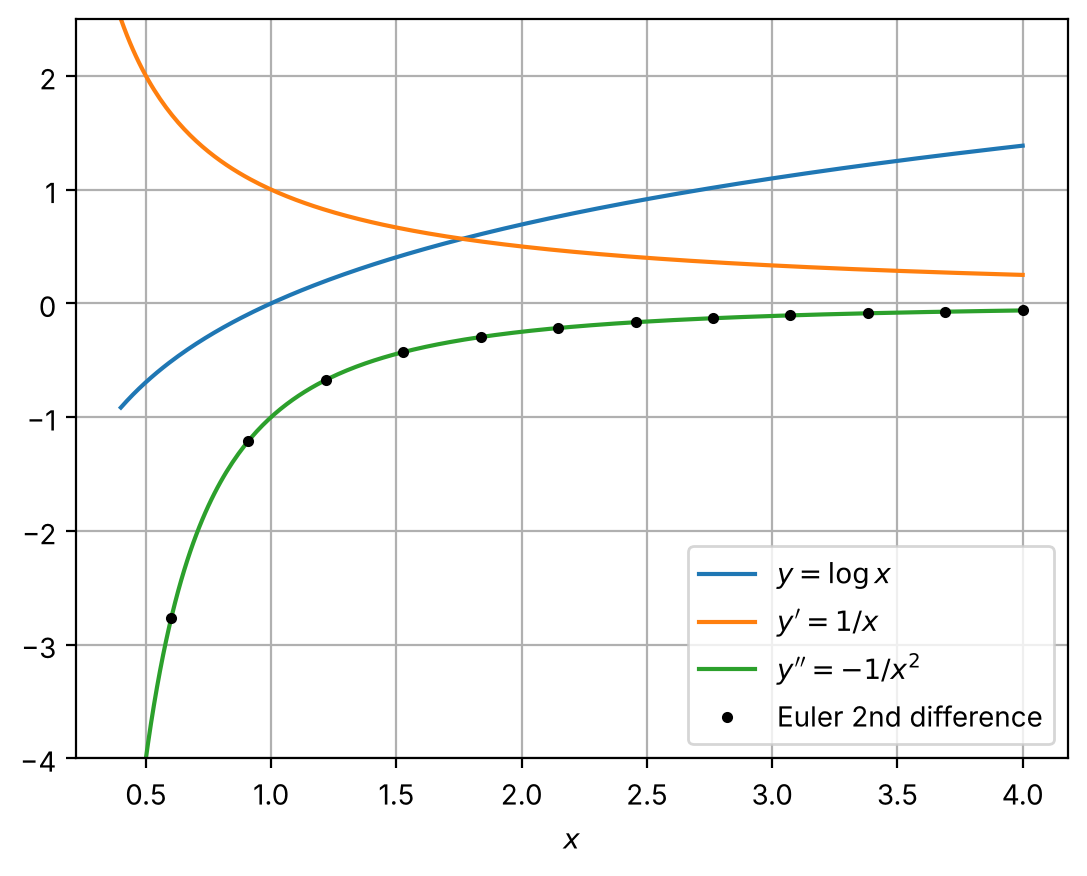
\includegraphics[width=0.65\linewidth]{figs/q15.png}
\caption{$y$, $y'$, $y''$ and the Euler second difference}
\label{fig:cb12-q15}
\end{figure}

\item Find the solution of the differential equation $\log\brak{\dfrac{dy}{dx}} = ax + by$.
\hfill (CBSE XII 65/C/3, Q17)

\solution $\frac{dy}{dx} = e^{ax}e^{by}$. Separating the variables,
\begin{align}
e^{-by}\,dy = e^{ax}\,dx \implies \frac{e^{ax}}{a} + \frac{e^{-by}}{b} = C
\end{align}
The equation is non-linear, so it is checked numerically. With $a = b = 1$ and $y(0) = 0$ (assumed) the solution is $e^x + e^{-y} = 2$, i.e. $y = -\log\brak{2 - e^x}$. The Euler forward method \eqref{eq:cb12-euler} with $500$ steps gives $y(0.5) = 1.0432$ against the exact $1.0462$. The Laplace derivative property \eqref{eq:cb12-lap1} on $[0, 0.5]$ is verified, $L\{e^{x+y}\} = sY - y(0) + e^{-sT}y(T)$, e.g. $0.583278$ at $s = 2$ on both sides. See \figref{fig:cb12-q17}.
\begin{lstlisting}[frame=single, basicstyle=\rmfamily, escapeinside={(*@}{@*)}]
(*@\makebox[\dimexpr\linewidth-2\fboxsep-2\fboxrule\relax][c]{codes/q17.py}@*)
\end{lstlisting}
\begin{figure}[H]
\centering
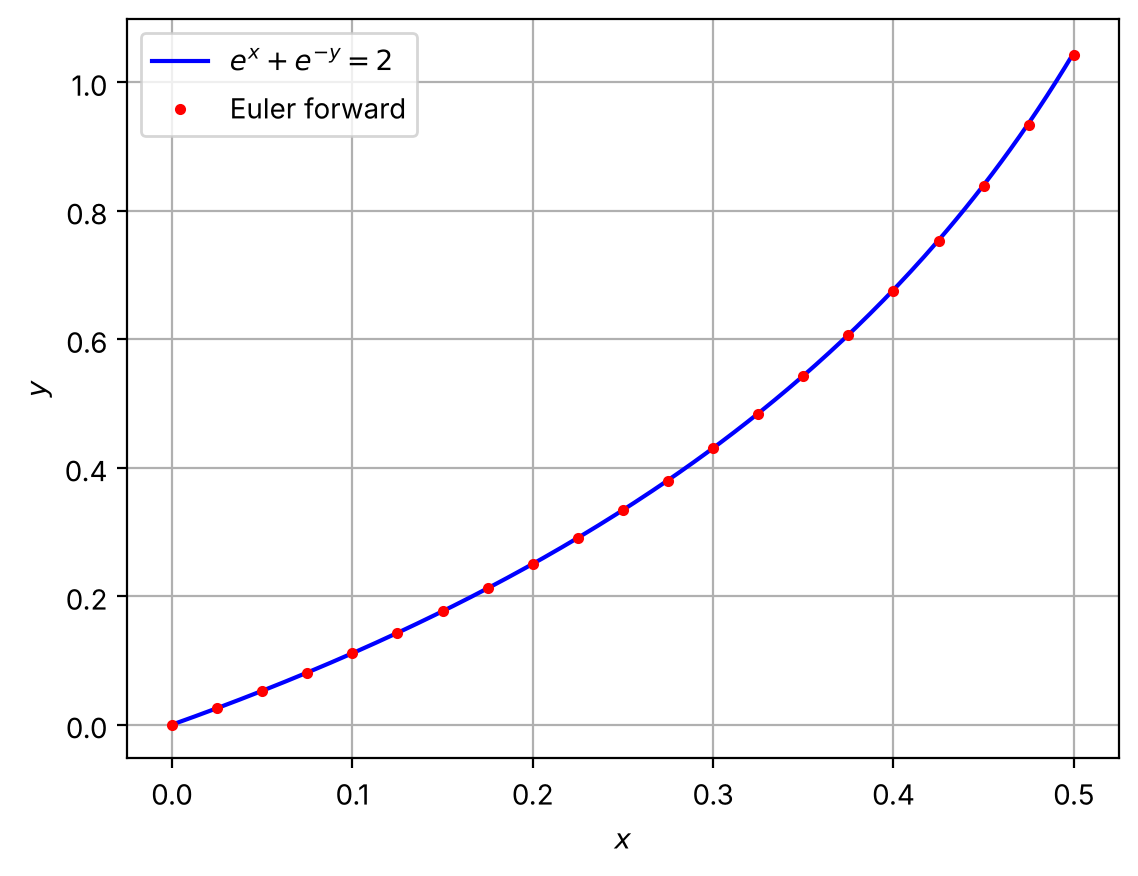
\includegraphics[width=0.55\linewidth]{figs/q17.png}
\caption{$e^x + e^{-y} = 2$ and the Euler forward method}
\label{fig:cb12-q17}
\end{figure}

\item If $\vec{a} = 2\hat{i} - \hat{j} + 2\hat{k}$ and $\vec{b} = 5\hat{i} - 3\hat{j} - 4\hat{k}$, then find the ratio $\dfrac{\text{projection of } \vec{a} \text{ on } \vec{b}}{\text{projection of } \vec{b} \text{ on } \vec{a}}$.
\hfill (CBSE XII 65/C/3, Q18)

\hfill OR \\
Let $\hat{a}$ and $\hat{b}$ be two unit vectors. If the vectors $\vec{c} = \hat{a} + 2\hat{b}$ and $\vec{d} = 5\hat{a} - 4\hat{b}$ are perpendicular to each other, then find the angle between $\hat{a}$ and $\hat{b}$.

\solution $\vec{a}^{\top}\vec{b} = 10 + 3 - 8 = 5$, $\norm{\vec{a}} = 3$, $\norm{\vec{b}} = \sqrt{50}$. From \eqref{eq:cb12-proj},
\begin{align}
\frac{\norm{\vec{a}}}{\norm{\vec{b}}} = \frac{3}{5\sqrt{2}}
\end{align}
\textbf{OR:} From \eqref{eq:cb12-dot}, $\vec{c}^{\top}\vec{d} = 5 - 4\cos\theta + 10\cos\theta - 8 = 6\cos\theta - 3 = 0$. Newton-Raphson \eqref{eq:cb12-nr} on $f\brak{\theta} = 6\cos\theta - 3$,
\begin{align}
\theta_{n+1} = \theta_n + \frac{6\cos\theta_n - 3}{6\sin\theta_n}
\end{align}
converges to $\theta = 60^\circ$. The following code verifies both parts.
\begin{lstlisting}[frame=single, basicstyle=\rmfamily, escapeinside={(*@}{@*)}]
(*@\makebox[\dimexpr\linewidth-2\fboxsep-2\fboxrule\relax][c]{codes/q18.py}@*)
\end{lstlisting}

\item Find the distance of the point $\brak{a,b,c}$ from the $x$-axis.
\hfill (CBSE XII 65/C/3, Q20)

\solution Let $\vec{P} = \myvec{a \\ b \\ c}$ and $\vec{e}_1 = \myvec{1 \\ 0 \\ 0}$. The foot of the perpendicular is $\brak{\vec{e}_1^{\top}\vec{P}}\vec{e}_1 = \myvec{a \\ 0 \\ 0}$ and from \ref{eq:cb12-axis},
\begin{align}
d = \norm{\vec{P} - a\vec{e}_1} = \norm{\myvec{0 \\ b \\ c}} = \sqrt{b^2 + c^2}
\end{align}
The following code verifies this for assumed points.
\begin{lstlisting}[frame=single, basicstyle=\rmfamily, escapeinside={(*@}{@*)}]
(*@\makebox[\dimexpr\linewidth-2\fboxsep-2\fboxrule\relax][c]{codes/q20.py}@*)
\end{lstlisting}

\item If $y = \sqrt{a + \sqrt{a + x}}$, then find $\dfrac{dy}{dx}$.
\hfill (CBSE XII 65/C/3, Q21)

\solution By the chain rule,
\begin{align}
\frac{dy}{dx} = \frac{1}{2\sqrt{a+\sqrt{a+x}}}\cdot\frac{1}{2\sqrt{a+x}} = \frac{1}{4\sqrt{a+x}\sqrt{a+\sqrt{a+x}}}
\end{align}
\textbf{Laplace transform:} with $a = 1$ (assumed) and $x \to t$, the property \eqref{eq:cb12-lap1} gives $L\{y'\} = sY(s) - y(0)$, $y(0) = \sqrt{2}$. The code computes $Y(s)$ by the trapezoidal rule: at $s = 2$, $L\{y'\} = 0.071386$ with $y'$ from the formula and $sY - y(0) = 0.071386$. The Euler forward difference \eqref{eq:cb12-euler-diff} gives $0.136853, 0.087324, 0.054952$ at $x = 0.5, 2, 5$, equal to the formula.
\begin{lstlisting}[frame=single, basicstyle=\rmfamily, escapeinside={(*@}{@*)}]
(*@\makebox[\dimexpr\linewidth-2\fboxsep-2\fboxrule\relax][c]{codes/q21.py}@*)
\end{lstlisting}

\item Show that the three vectors $2\hat{i} - \hat{j} + \hat{k}$, $\hat{i} - 3\hat{j} - 5\hat{k}$ and $3\hat{i} - 4\hat{j} - 4\hat{k}$ form the vertices of a right-angled triangle.
\hfill (CBSE XII 65/C/3, Q22)

\solution Let $\vec{A} = \myvec{2 \\ -1 \\ 1}$, $\vec{B} = \myvec{1 \\ -3 \\ -5}$, $\vec{C} = \myvec{3 \\ -4 \\ -4}$. Then
\begin{align}
\vec{B}-\vec{C} = \myvec{-2 \\ 1 \\ -1}, \quad \vec{A}-\vec{C} = \myvec{-1 \\ 3 \\ 5}
\implies \brak{\vec{B}-\vec{C}}^{\top}\brak{\vec{A}-\vec{C}} = 2 + 3 - 5 = 0
\end{align}
so $\angle C = 90^\circ$. Also $BC^2 + CA^2 = 6 + 35 = 41 = AB^2$. The following code verifies this.
\begin{lstlisting}[frame=single, basicstyle=\rmfamily, escapeinside={(*@}{@*)}]
(*@\makebox[\dimexpr\linewidth-2\fboxsep-2\fboxrule\relax][c]{codes/q22.py}@*)
\end{lstlisting}

\item A bag contains $19$ tickets, numbered $1$ to $19$. A ticket is drawn at random and then another ticket is drawn without replacing the first one. Find the probability distribution of the number of even numbers on the ticket.
\hfill (CBSE XII 65/C/3, Q23)

\hfill OR \\
Find the probability distribution of the number of successes in two tosses of a die, when a success is defined as ``number greater than $5$''.

\solution There are $9$ even and $10$ odd tickets. Let $X$ be the number of even tickets in the two draws. The ordered pairs are $19\cdot 18 = 342$ equally likely outcomes, so
\begin{align}
p_X(0) = \frac{10\cdot 9}{342} = \frac{5}{19}, \quad p_X(1) = \frac{2\cdot 9\cdot 10}{342} = \frac{10}{19}, \quad p_X(2) = \frac{9\cdot 8}{342} = \frac{4}{19}
\end{align}
and $\frac{5+10+4}{19} = 1$ as required by \eqref{eq:cb12-pmf}.

\textbf{OR:} The success probability is $\pr{6} = \frac{1}{6}$. For one toss the pmf is $\myvec{\frac{5}{6} & \frac{1}{6}}$; for two tosses, by convolution,
\begin{align}
p_X = \myvec{\frac{5}{6} & \frac{1}{6}} * \myvec{\frac{5}{6} & \frac{1}{6}} = \myvec{\frac{25}{36} & \frac{10}{36} & \frac{1}{36}}
\end{align}
The following code enumerates both in \figref{fig:cb12-q23}.
\begin{lstlisting}[frame=single, basicstyle=\rmfamily, escapeinside={(*@}{@*)}]
(*@\makebox[\dimexpr\linewidth-2\fboxsep-2\fboxrule\relax][c]{codes/q23.py}@*)
\end{lstlisting}
\begin{figure}[H]
\centering
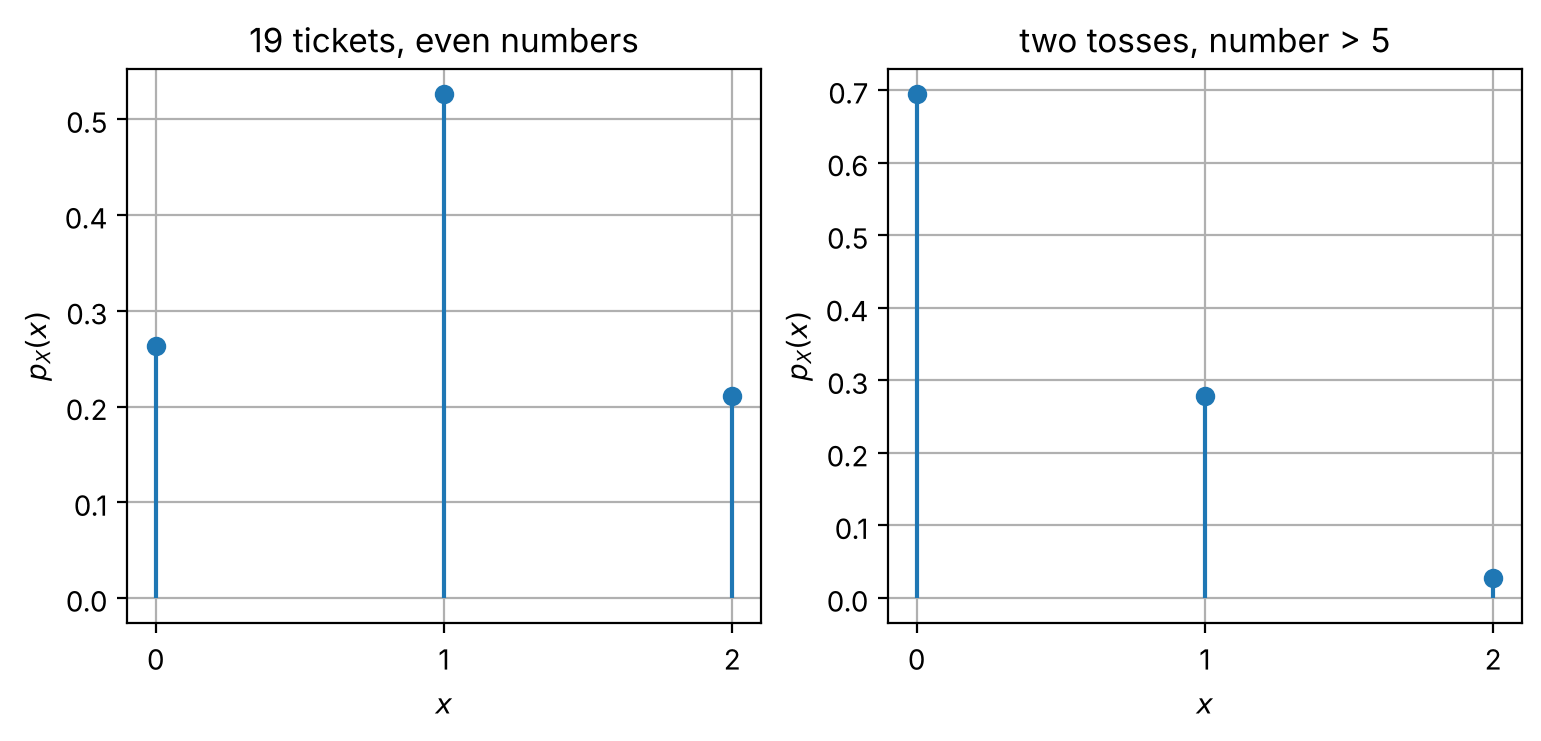
\includegraphics[width=0.80\linewidth]{figs/q23.png}
\caption{pmfs for the tickets (left) and for the die (right)}
\label{fig:cb12-q23}
\end{figure}

\item Solve the following homogeneous differential equation: $x\dfrac{dy}{dx} = x + y$.
\hfill (CBSE XII 65/C/3, Q26)

\solution Put $x = e^t$, so $x\frac{dy}{dx} = \frac{dy}{dt}$ and the equation is $\frac{dy}{dt} - y = e^t$. Taking the Laplace transform from \eqref{eq:cb12-lap1} and \eqref{eq:cb12-laplace},
\begin{align}
sY - y_0 - Y = \frac{1}{s-1} \implies Y(s) = \frac{y_0}{s-1} + \frac{1}{\brak{s-1}^2}
\end{align}
Inverting, $y = \brak{y_0 + t}e^t$, i.e.
\begin{align}
y = x\brak{\log x + C}
\end{align}
The code checks that the numerical transform of $\brak{C+t}e^t$ equals $Y(s)$ (for $C = 0.5$, $s = 3$: $0.5$ on both sides) and solves the equation by the Euler forward method \eqref{eq:cb12-euler}: at $x = 4$ it gives $7.5302$ against $7.5452$. See \figref{fig:cb12-q26}.
\begin{lstlisting}[frame=single, basicstyle=\rmfamily, escapeinside={(*@}{@*)}]
(*@\makebox[\dimexpr\linewidth-2\fboxsep-2\fboxrule\relax][c]{codes/q26.py}@*)
\end{lstlisting}
\begin{figure}[H]
\centering
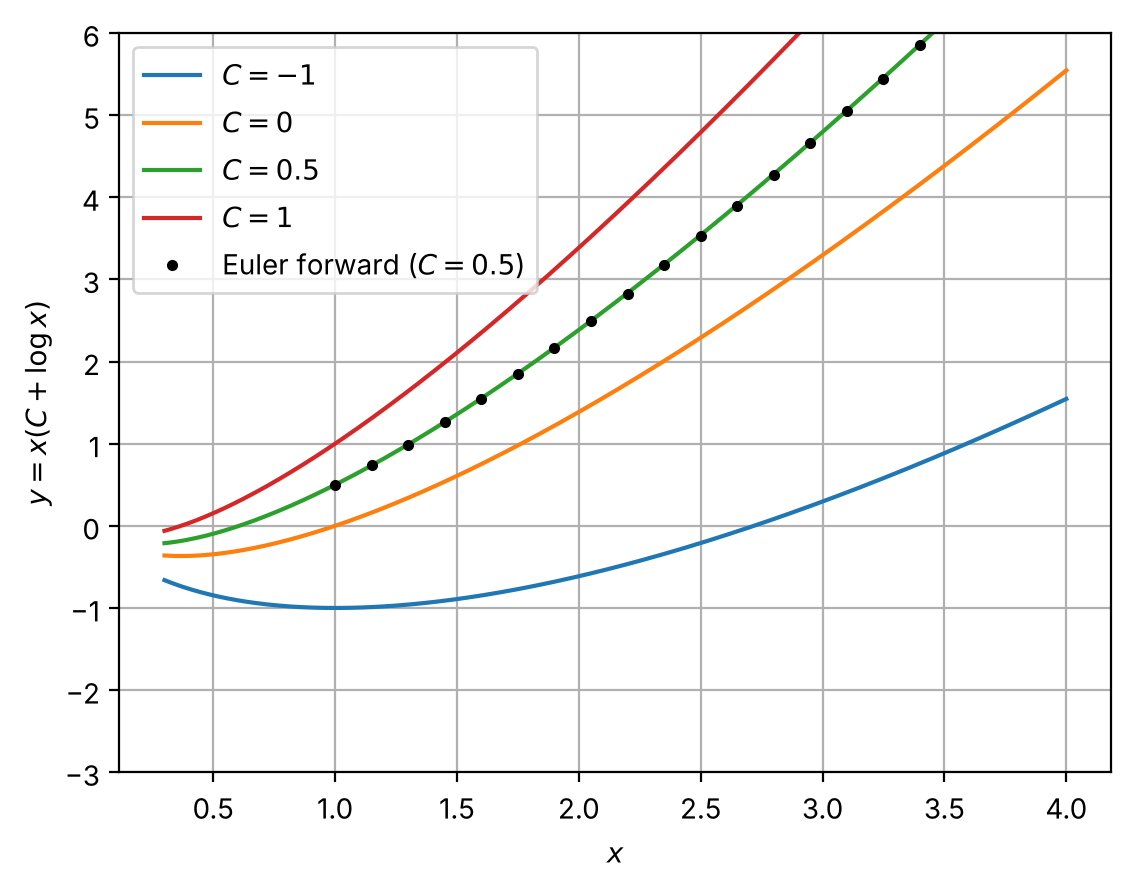
\includegraphics[width=0.65\linewidth]{figs/q26.png}
\caption{Solutions $y = x(C + \log x)$ and the Euler forward method}
\label{fig:cb12-q26}
\end{figure}

\item The random variable $X$ has a probability function $P(x)$ defined below, where $k$ is some number: $P(x) = k$ for $x = 0$, $2k$ for $x = 1$, $3k$ for $x = 2$, and $0$ otherwise. Find (i) the value of $k$, (ii) $P(X < 2)$, $P(X \le 2)$, $P(X \ge 2)$.
\hfill (CBSE XII 65/C/3, Q28)

\solution From \eqref{eq:cb12-pmf} the pmf sums to $1$: $\myvec{1 & 2 & 3}\myvec{k \\ k \\ k} = 6k = 1$, so $k = \frac{1}{6}$ (Gauss elimination on the $1\times 1$ system). The pmf is $\myvec{\frac{1}{6} & \frac{2}{6} & \frac{3}{6}}$ and
\begin{align}
P(X<2) &= \frac{1}{6} + \frac{2}{6} = \frac{1}{2}, \quad P(X \le 2) = 1, \quad P(X \ge 2) = \frac{3}{6} = \frac{1}{2}
\end{align}
The following code verifies this in \figref{fig:cb12-q28}.
\begin{lstlisting}[frame=single, basicstyle=\rmfamily, escapeinside={(*@}{@*)}]
(*@\makebox[\dimexpr\linewidth-2\fboxsep-2\fboxrule\relax][c]{codes/q28.py}@*)
\end{lstlisting}
\begin{figure}[H]
\centering
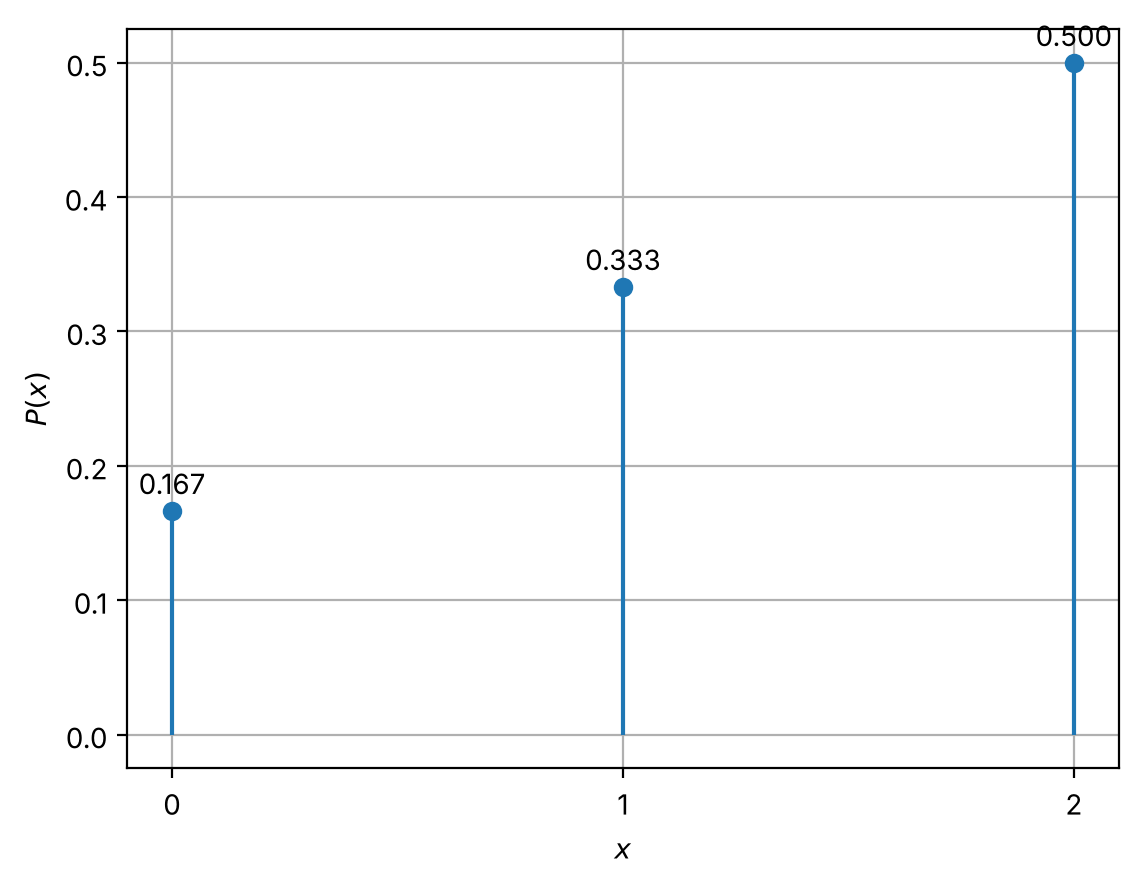
\includegraphics[width=0.50\linewidth]{figs/q28.png}
\caption{pmf of $X$}
\label{fig:cb12-q28}
\end{figure}

\item Find the shortest distance between the following lines and hence write whether the lines are intersecting or not: $\dfrac{x-1}{2} = \dfrac{y+1}{3} = z$, $\dfrac{x+1}{5} = \dfrac{y-2}{1}$, $z = 2$.
\hfill (CBSE XII 65/C/3, Q30)

\hfill OR \\
Find the equation of the plane through the line of intersection of the planes $\vec{r}\cdot\brak{\hat{i} + 3\hat{j}} + 6 = 0$ and $\vec{r}\cdot\brak{3\hat{i} - \hat{j} - 4\hat{k}} = 0$, which is at a unit distance from the origin.

\solution $\vec{p}_1 = \myvec{1 \\ -1 \\ 0}$, $\vec{d}_1 = \myvec{2 \\ 3 \\ 1}$, $\vec{p}_2 = \myvec{-1 \\ 2 \\ 2}$, $\vec{d}_2 = \myvec{5 \\ 1 \\ 0}$, $\vec{w} = \vec{p}_1 - \vec{p}_2 = \myvec{2 \\ -3 \\ -2}$. The normal equations \eqref{eq:cb12-skew} are
\begin{align}
\myvec{14 & -13 \\ 13 & -26}\myvec{s \\ t} = \myvec{-\brak{4 - 9 - 2} \\ -\brak{10 - 3}} = \myvec{7 \\ -7}
\end{align}
Gauss elimination, $R_2 \leftarrow R_2 - \frac{13}{14}R_1$:
\begin{align}
\myvec{14 & -13 & 7 \\ 13 & -26 & -7} \longrightarrow \myvec{14 & -13 & 7 \\ 0 & -\frac{195}{14} & -\frac{189}{14}}
\implies t = \frac{189}{195} = \frac{63}{65}, \quad s = \frac{7 + 13t}{14} = \frac{7}{5}
\end{align}
The closest points are $\vec{p}_1 + s\vec{d}_1 = \myvec{3.8 \\ 3.2 \\ 1.4}$ and $\vec{p}_2 + t\vec{d}_2 = \myvec{3.846 \\ 2.969 \\ 2}$. The shortest distance is
\begin{align}
d = \norm{\brak{\vec{p}_1 + s\vec{d}_1} - \brak{\vec{p}_2 + t\vec{d}_2}} = \frac{9}{\sqrt{195}} \approx 0.6445 \neq 0
\end{align}
so the lines do not intersect.

\textbf{OR:} The planes are $\vec{n}_1 = \myvec{1 \\ 3 \\ 0}$, $c_1 = -6$ and $\vec{n}_2 = \myvec{3 \\ -1 \\ -4}$, $c_2 = 0$. From \eqref{eq:cb12-family}, $\vec{n} = \myvec{1+3\lambda \\ 3-\lambda \\ -4\lambda}$, $c = -6$ and the distance condition $\frac{6}{\norm{\vec{n}}} = 1$ gives
\begin{align}
g\brak{\lambda} = \norm{\vec{n}}^2 - 36 = 26\lambda^2 - 26 = 0
\end{align}
The Newton-Raphson iteration \eqref{eq:cb12-nr}, $\lambda_{n+1} = \lambda_n - \frac{g\brak{\lambda_n}}{52\lambda_n}$, gives $\lambda = \pm 1$ and the planes
\begin{align}
4x + 2y - 4z + 6 = 0, \quad -2x + 4y + 4z + 6 = 0
\end{align}
i.e. $2x + y - 2z + 3 = 0$ and $x - 2y - 2z - 3 = 0$. The following code verifies both parts.
\begin{lstlisting}[frame=single, basicstyle=\rmfamily, escapeinside={(*@}{@*)}]
(*@\makebox[\dimexpr\linewidth-2\fboxsep-2\fboxrule\relax][c]{codes/q30.py}@*)
\end{lstlisting}

\item Find a unit vector perpendicular to each of the vectors $\brak{\vec{a}+\vec{b}}$ and $\brak{\vec{a}-\vec{b}}$ where $\vec{a} = \hat{i} + \hat{j} + \hat{k}$, $\vec{b} = \hat{i} + 2\hat{j} + 3\hat{k}$.
\hfill (CBSE XII 65/C/3, Q31)

\solution $\vec{u} = \vec{a}+\vec{b} = \myvec{2 \\ 3 \\ 4}$, $\vec{v} = \vec{a}-\vec{b} = \myvec{0 \\ -1 \\ -2}$. From \ref{eq:cb12-perp}, with $n_3 = 1$,
the augmented matrix (rows $\vec{u}^{\top}$ and $\vec{v}^{\top}$, right side $-u_3, -v_3$) is already upper triangular:
\begin{align}
\myvec{2 & 3 & -4 \\ 0 & -1 & 2}
\end{align}
Back substitution: $-n_2 = 2 \implies n_2 = -2$, $2n_1 + 3\brak{-2} = -4 \implies n_1 = 1$. So $\vec{n} = \myvec{1 \\ -2 \\ 1}$, $\norm{\vec{n}} = \sqrt{6}$ and the unit vectors are
\begin{align}
\pm\frac{1}{\sqrt{6}}\myvec{1 \\ -2 \\ 1}
\end{align}
The following code verifies $\vec{n}^{\top}\vec{u} = \vec{n}^{\top}\vec{v} = 0$.
\begin{lstlisting}[frame=single, basicstyle=\rmfamily, escapeinside={(*@}{@*)}]
(*@\makebox[\dimexpr\linewidth-2\fboxsep-2\fboxrule\relax][c]{codes/q31.py}@*)
\end{lstlisting}

\item Using properties of determinants show that
\begin{align*}
\mydet{1+a^2-b^2 & 2ab & -2b \\ 2ab & 1-a^2+b^2 & 2a \\ 2b & -2a & 1-a^2-b^2} = \brak{1+a^2+b^2}^3
\end{align*}
\hfill (CBSE XII 65/C/3, Q32)

\hfill OR \\
Find the equation of the line joining $A\brak{1,3}$ and $B\brak{0,0}$ using determinants. Also, find $k$ if $D\brak{k,0}$ is a point such that the area of $\triangle ABD$ is $3$ square units.

\solution Apply $R_1 \leftarrow R_1 + bR_3$ and $R_2 \leftarrow R_2 - aR_3$ (the determinant is unchanged, from \eqref{eq:cb12-det}). With $\Delta = 1 + a^2 + b^2$,
\begin{align}
\mydet{\Delta & 0 & -b\Delta \\ 0 & \Delta & a\Delta \\ 2b & -2a & 1-a^2-b^2} &= \Delta^2\mydet{1 & 0 & -b \\ 0 & 1 & a \\ 2b & -2a & 1-a^2-b^2}
\end{align}
Expanding the last determinant along the first row,
\begin{align}
\brak{1 - a^2 - b^2 + 2a^2} + \brak{-b}\brak{0 - 2b} = 1 + a^2 + b^2 = \Delta
\end{align}
so the value is $\Delta^3 = \brak{1+a^2+b^2}^3$. $\blacksquare$ The code checks it by cofactor expansion for random $a, b$.

\textbf{OR:} $\vec{n} = \myvec{0 & 1 \\ -1 & 0}\brak{\vec{A}-\vec{B}} = \myvec{3 \\ -1}$ and the line is $\vec{n}^{\top}\vec{x} = 0$, i.e. $3x - y = 0$. From \eqref{eq:cb12-area}, the area is $\frac{1}{2}\abs{\vec{n}^{\top}\myvec{k \\ 0}} = \frac{3\abs{k}}{2} = 3$, so $k = \pm 2$. The following code verifies this.
\begin{lstlisting}[frame=single, basicstyle=\rmfamily, escapeinside={(*@}{@*)}]
(*@\makebox[\dimexpr\linewidth-2\fboxsep-2\fboxrule\relax][c]{codes/q32.py}@*)
\end{lstlisting}

\item Evaluate $\displaystyle\int_1^3\brak{x^2 + 1 + e^x}dx$ as the limit of sums.
\hfill (CBSE XII 65/C/3, Q34)

\solution With $h = \frac{2}{n}$ and $f(x) = x^2 + 1 + e^x$,
\begin{align}
\int_1^3 f\,dx &= \lim_{n\to\infty}h\sum_{i=1}^{n}f\brak{1+ih} \\
&= \lim_{n\to\infty}h\sbrak{2n + 2h\frac{n\brak{n+1}}{2} + h^2\frac{n\brak{n+1}\brak{2n+1}}{6} + e\frac{e^h\brak{e^{nh}-1}}{e^h - 1}}
\end{align}
Using $nh = 2$ and $\frac{h}{e^h-1} \to 1$, the limit is $4 + 4 + \frac{8}{3} + e\brak{e^2 - 1}$, so
\begin{align}
\int_1^3 f\,dx &= \frac{32}{3} + e^3 - e \approx 28.03392
\end{align}
The trapezoidal rule \eqref{eq:cb12-trap} gives $28.4776$ for $N = 4$, $28.0357$ for $N = 64$ and $28.03392$ for $N = 16384$, converging to the same value. The following code verifies this.
\begin{lstlisting}[frame=single, basicstyle=\rmfamily, escapeinside={(*@}{@*)}]
(*@\makebox[\dimexpr\linewidth-2\fboxsep-2\fboxrule\relax][c]{codes/q34.py}@*)
\end{lstlisting}

\item If $y = x^{\sin x} + \sin^{-1}\sqrt{x}$, then find $\dfrac{dy}{dx}$.
\hfill (CBSE XII 65/C/3, Q36)

\solution Let $y_1 = x^{\sin x}$, so $\log y_1 = \sin x\log x$ and $\frac{y_1'}{y_1} = \cos x\log x + \frac{\sin x}{x}$. Also $\frac{d}{dx}\sin^{-1}\sqrt{x} = \frac{1}{\sqrt{1-x}}\cdot\frac{1}{2\sqrt{x}}$. Hence
\begin{align}
\frac{dy}{dx} = x^{\sin x}\brak{\cos x\log x + \frac{\sin x}{x}} + \frac{1}{2\sqrt{x\brak{1-x}}}
\end{align}
\textbf{Laplace transform:} on $x = 0.25 + t$, $t \in \sbrak{0, 0.5}$, the property \eqref{eq:cb12-lap1} on a finite interval reads $L\{y'\} = sY(s) - y(0) + e^{-sT}y(T)$. The code evaluates $Y(s)$ with the trapezoidal rule: at $s = 2$ both sides equal $0.381810$; at $s = 5$ both equal $0.206807$. The Euler forward difference \eqref{eq:cb12-euler-diff} gives $0.975397, 1.251443, 1.605675$ at $x = 0.3, 0.5, 0.7$ against the formula values $0.975396, 1.251442, 1.605674$.
\begin{lstlisting}[frame=single, basicstyle=\rmfamily, escapeinside={(*@}{@*)}]
(*@\makebox[\dimexpr\linewidth-2\fboxsep-2\fboxrule\relax][c]{codes/q36.py}@*)
\end{lstlisting}

\end{enumerate}
